\documentclass[14pt]{beamer}
\usepackage[T1]{fontenc}
\usepackage{tikz}
\usepackage[quiet]{mathspec}
\usepackage{ifthen}

\usetikzlibrary{matrix,arrows.meta}
 % Tells beamer that math mode should use serif fonts
\usefonttheme[onlymath]{serif}

% Sets the serif font (which is the main font)
\setmainfont{Linux Libertine O}

% Sets the font beamer uses, which is sans-serif by default
\setsansfont[
ItalicFont={YanoneKaffeesatz-Light},
Scale=1.3,
LetterSpace=2.0
]{YanoneKaffeesatz-Bold}

% Replaces every explicit \mathrm call to use this font
\setmathrm{Linux Libertine O}

% The base16 colour scheme?
\definecolor{sbase03}{HTML}{002B36}
\definecolor{sbase02}{HTML}{073642}
\definecolor{sbase01}{HTML}{586E75}
\definecolor{sbase00}{HTML}{657B83}
\definecolor{sbase0}{HTML}{839496}
\definecolor{sbase1}{HTML}{93A1A1}
\definecolor{sbase2}{HTML}{EEE8D5}
\definecolor{sbase3}{HTML}{FDF6E3}
\definecolor{syellow}{HTML}{B58900}
\definecolor{sorange}{HTML}{CB4B16}
\definecolor{sred}{HTML}{DC322F}
\definecolor{smagenta}{HTML}{D33682}
\definecolor{sviolet}{HTML}{6C71C4}
\definecolor{sblue}{HTML}{268BD2}
\definecolor{scyan}{HTML}{2AA198}
\definecolor{sgreen}{HTML}{859900}

\definecolor{Tropiteal}{RGB}{0,168,198}
\definecolor{TealDrop}{RGB}{64,192,203}
\definecolor{WhiteTrash}{RGB}{249,242,231}
\definecolor{AtomicBikini}{RGB}{174,226,57}
\definecolor{FeebleWeek}{RGB}{143,190,0}
\definecolor{ICantExpress}{RGB}{28,20,13}
\definecolor{Marty}{RGB}{250,42,0}

\colorlet{ColourBase}{Tropiteal}
\colorlet{ColourHl1}{Marty}
\colorlet{ColourHl2}{FeebleWeek}
\colorlet{ColourHl3}{TealDrop}
\colorlet{ColourDark}{ICantExpress}
\colorlet{ColourDark2}{Tropiteal}


\usetheme{metropolis}

\setbeamercolor{alerted text}{%
  fg=bazelGreen
}

\setbeamercolor{example text}{%
  fg=mLightBrown
}

\setbeamercolor{frametitle}{%
  use=normal text,
  fg=normal text.bg,
  bg=bazelGreen
}

\lstset{%
  basicstyle=\ttfamily\lst@ifdisplaystyle\fontsize{9pt}{9pt}\selectfont\fi,
  keywordstyle=\color{sgreen}, identifierstyle=\color{sblue}, 
  commentstyle=\color{sbase1}, stringstyle=\color{sorange},
  numberstyle=\color{sviolet}, showstringspaces=false,  
  breaklines=true,
  tabsize=5,
}

\lstalias[]{gnumake}[gnu]{make}




\usetikzlibrary{fadings,decorations.pathmorphing}
% Code courtesy of https://tex.stackexchange.com/a/137438/39313

\makeatletter
\newif\iftikz@shading@path

\tikzset{
    % There are three circumstances in which the fading sep is needed:
    % 1. Arrows which do not update the bounding box (which is most of them).
    % 2. Line caps/joins and mitres that extend outside the natural bounding 
    %    box of the path (these are not calculated by PGF).
    % 3. Other reasons that haven't been anticipated.
    shading xsep/.store in=\tikz@pathshadingxsep,
    shading ysep/.store in=\tikz@pathshadingysep,
    shading sep/.style={shading xsep=#1, shading ysep=#1},
    shading sep=0.0cm,
}

\def\tikz@shadepath#1{% 
    % \tikz@addmode installs the `modes' (e.g., fill, draw, shade) 
    % to be applied to the path. It isn't usualy for doing more
    % changes to the path's construction.
    \iftikz@shading@path%
    \else%
        \tikz@shading@pathtrue%
        % Get the current path.
        \pgfgetpath\tikz@currentshadingpath%
        % Get the shading sep without setting any other keys.
        \begingroup%
            \pgfsys@beginscope% <- may not be necessary
            \tikzset{#1}%
            \xdef\tikz@tmp{\noexpand\def\noexpand\tikz@pathshadingxsep{\tikz@pathshadingxsep}%
                \noexpand\def\noexpand\tikz@pathshadingysep{\tikz@pathshadingysep}}%
            \pgfsys@endscope%
        \endgroup
        \tikz@tmp%
        % Get the boudning box of the current path size including the shading sep
        \pgfextract@process\pgf@shadingpath@southwest{\pgfpointadd{\pgfqpoint{\pgf@pathminx}{\pgf@pathminy}}%
            {\pgfpoint{-\tikz@pathshadingxsep}{-\tikz@pathshadingysep}}}%%
        \pgfextract@process\pgf@shadingpath@northeast{\pgfpointadd{\pgfqpoint{\pgf@pathmaxx}{\pgf@pathmaxy}}%
            {\pgfpoint{\tikz@pathshadingxsep}{\tikz@pathshadingysep}}}%
        % Clear the path
        \pgfsetpath\pgfutil@empty%                          
        % Save the current drawing mode and options.
        \let\tikz@options@saved=\tikz@options%
        \let\tikz@mode@saved=\tikz@mode%
        \let\tikz@options=\pgfutil@empty%
        \let\tikz@mode=\pgfutil@empty%
        % \tikz@options are processed later on.
        \tikz@addoption{%
            \pgfinterruptpath%
            \pgfinterruptpicture%
                \begin{tikzfadingfrompicture}[name=.]
                \pgfscope%
                    \tikzset{shade path/.style=}% Make absolutely sure shade path is not inherited.
                    \path \pgfextra{%
                        % Set the softpath. Any transformations,draw=none} in #1 will have no effect.
                        % This will *not* update the bounding box...
                        \pgfsetpath\tikz@currentshadingpath%
                        % ...so it is done manually.
                        \pgf@shadingpath@southwest
                        \expandafter\pgf@protocolsizes{\the\pgf@x}{\the\pgf@y}%
                        \pgf@shadingpath@northeast%
                        \expandafter\pgf@protocolsizes{\the\pgf@x}{\the\pgf@y}%
                        % Install the drawing modes and options.
                        \let\tikz@options=\tikz@options@saved%
                        \let\tikz@mode=\tikz@mode@saved%
                    };
                    % Now get the bounding box of the picture.
                    \xdef\pgf@shadingboundingbox@southwest{\noexpand\pgfqpoint{\the\pgf@picminx}{\the\pgf@picminy}}%
                    \xdef\pgf@shadingboundingbox@northeast{\noexpand\pgfqpoint{\the\pgf@picmaxx}{\the\pgf@picmaxy}}%
                    \endpgfscope
                \end{tikzfadingfrompicture}%
            \endpgfinterruptpicture%
            \endpgfinterruptpath%
            % Install a rectangle that covers the shaded/faded path picture.
            \pgftransformreset%
            \pgfpathrectanglecorners{\pgf@shadingboundingbox@southwest}{\pgf@shadingboundingbox@northeast}%
            %
            % Reset all modes.
            \let\tikz@path@picture=\pgfutil@empty%
            \tikz@mode@fillfalse%
            \tikz@mode@drawfalse%
            \tikz@mode@doublefalse%
            \tikz@mode@clipfalse%
            \tikz@mode@boundaryfalse%
            \tikz@mode@fade@pathfalse%
            \tikz@mode@fade@scopefalse%
            % Now install shading options.
            \tikzset{#1}%
            \tikz@mode%
            % Make the fading happen.
            \def\tikz@path@fading{.}%
            \tikz@mode@fade@pathtrue%
            \tikz@fade@adjustfalse%
            % Shift the fading to the mid point of the rectangle
            \pgfpointscale{0.5}{\pgfpointadd{\pgf@shadingboundingbox@southwest}{\pgf@shadingboundingbox@northeast}}%
            \edef\tikz@fade@transform{shift={(\the\pgf@x,\the\pgf@y)}}%
            \pgfsetfading{\tikz@path@fading}{\tikz@do@fade@transform}%
            \tikz@mode@fade@pathfalse%              
        }%
    \fi%
}
\tikzset{
    shade path/.code={%
        \tikz@addmode{\tikz@shadepath{#1}}%
    }
}

\makeatother


\newcommand{\minipos}[4]{\scalebox{0.5}{$\{#1, #2, #3, #4\}$}}
\def\clap#1{\hbox to 0pt{\hss#1\hss}}
\newcommand{\tikzmark}[1]{\tikz[overlay,remember picture] \coordinate (#1);}
\def\colours{{"Marty","FeebleWeek","Tropiteal"}}

\usetikzlibrary{decorations}
\usetikzlibrary{decorations.markings,decorations.pathmorphing,decorations.pathreplacing}

\tikzset{
  lattice-gluon/.style={
    draw=ICantExpress, thick,
    decoration={coil, amplitude=4pt, segment length=4pt},
    decorate,
  },
}

\usefonttheme{serif}
\setbeamertemplate{footline}{}

\title{Squeezing water from a stone}
\subtitle{A brief overview of lattice QCD}
\author{\texorpdfstring{%
    Aleksandra Rylund Glesaaen\newline%
    \fontsize{12pt}{12pt}\selectfont\texttt{aleksandra@glesaaen.com}%
    }{%
Aleksandra Rylund Glesaaen}}

\date{April 19th 2021}

\begin{document}

\maketitle

\section{A bit about me}
\frame{\sectionpage}

\begin{frame}{Background}

  \begin{itemize}
    \setlength{\itemsep}{20pt}
    \item NTNU: Master's in physics
    \item Frankfurt: PhD in Lattice QCD
    \item Swansea: Postdoc Lattice QCD
    \item Oslo: Software development
  \end{itemize}
  
\end{frame}

\section{Lattice QCD}
\frame{\sectionpage}

\begin{frame}[fragile]
  \frametitle{Quantum Chromo Dynamics}

  Theoretical description of the {\color{FeebleWeek}strong nuclear force}
  \vspace{1cm}

  \begin{center}
    \begin{tikzpicture}
      \node[circle,draw,thick,minimum size=1.5cm,fill=Tropiteal, fill opacity=0.5, text opacity=1.0] (q) {\strut{}q};
      \node[circle,draw,thick,minimum size=1.5cm,fill=Marty, fill opacity=0.5, text opacity=1.0] (qbar) at (5,0) {\strut{}q};
      
      \path[
        draw=transparent!0, very thick,
        shade path={left color=Tropiteal, right color=Marty},
        decoration={coil, amplitude=7pt, segment length=7pt, pre length=2pt, post length=2pt},
        decorate,
      ] (q) -- (qbar);
      
      \draw[thick, transform canvas={yshift=-7pt}] ([xshift=11pt] qbar.north west) -- ([xshift=-11pt] qbar.north east);
    \end{tikzpicture}
  \end{center}

  \vspace{1em}

  It binds matter together at the subatomic level
\end{frame}

\begin{frame}{Lattice QCD}

  Basically we just put on a {\large{}({\color{Marty}HUGE})} lattice

  \begin{center}
    \includegraphics{figures/lattice_conceptual.pdf}
  \end{center}

\end{frame}

\begin{frame}{The important equations}

  \begin{equation*}
    S = \int \mathrm{d}^4 x \, \bar{\psi}(x) Q\, \psi(x) + \mathcal{L}_g[U(x)] \end{equation*}

  \onslide<2->{%
  \begin{equation*}
    \mathcal{Z} = \int \mathrm{D} \psi \mathrm{D} U \, e^{-S[\psi,U\,]}
  \end{equation*}}

  \vspace*{-0.2cm}

  \onslide<3>{%
  \begin{equation*}
    \langle \mathcal{O} \rangle = \frac{1}{\mathcal{Z}} \int \mathrm{D} \psi \mathrm{D} U \, \mathcal{O}[\psi,U\,] \, e^{-S[\psi,U\,]}
  \end{equation*}}

\end{frame}

\begin{frame}{Discretisation}

  \begin{equation*}
    S \to \sum_{i,j} \bar{\psi}(x_i) Q_{i,j}[U\,]\, \psi(x_j) + \mathcal{L}_g[U(x_i)]
  \end{equation*}

  \onslide<2->{%
  \begin{equation*}
    \mathcal{Z} = \int \mathrm{D} \psi \mathrm{D} U \, e^{-S[\psi,U\,]} =
    \int\mathrm{D} U\, \mathrm{det}(Q) e^{-\sum \mathcal{L}_g[U(x)]}
  \end{equation*}}

\end{frame}

\section{Monte Carlo Integration}
\frame{\sectionpage}

\begin{frame}{Monte Carlo integration}

  \begin{center}
    \includegraphics[scale=2.2]{figures/monte_carlo_integrals.pdf}
  \end{center}

\end{frame}

\begin{frame}{The QCD Integrand}
  \begin{center}
    \includegraphics{figures/action_multiple_peaks.pdf}
  \end{center}
\end{frame}

\begin{frame}{The QCD Integrand}
  \begin{center}
    \includegraphics{figures/action_mc_itegral.pdf}
  \end{center}
\end{frame}

\begin{frame}{Redefining the problem}

  \vspace*{-1cm}

  \begin{equation*}
    \langle \mathcal{O} \rangle = \int \mathrm{D} U \, \mathcal{O}[U\,]
    \begin{tikzpicture}[baseline={(trace.base)}]
      \node[inner sep=0pt] (trace) {%
        $\displaystyle\frac{1}{\mathcal{Z}} e^{-S[U\,]}$};
      \draw [
        decorate,
        line width=1.4pt,
        decoration={
          brace,
          mirror,
          amplitude=5pt
        },
      ]
        ([yshift=-.2cm]trace.south west) -- ([yshift=-.2cm]trace.south east)
        node[midway,below=5pt] {\clap{Probability density}};
    \end{tikzpicture}
    = \int \mathrm{D} U \, \mathcal{O}[U\,] \mathcal{P}[U\,]
  \end{equation*}

  Integral over U can be stochastically estimated.

  \begin{equation*}
    \langle\mathcal{O}\,\rangle \approx  \frac{1}{N} \sum_k
    \mathcal{O}[U_k]\tikzmark{eoq}\hspace{1cm}
  \end{equation*}

    \nointerlineskip
    \begin{tikzpicture}[overlay,remember picture]
      \draw[{Stealth}-] ([shift={(-3.1mm,-2mm)}] eoq) -- ++(0,-5mm) -- +(0.5cm,0)
        node[right,scale=0.8,align=left,font=\fontspec{YanoneKaffeesatz-Light}] {Distributed $\propto \mathcal{P}$};
    \end{tikzpicture}

\end{frame}

\begin{frame}{Markov Chains}

  \begin{center}
  \begin{tikzpicture}

    \node (U1) {$U_1$};
    \node (U2) [right=of U1] {$U_2$};
    \node (U3) [right=of U2] {$U_3$};
    \node (U4) [right=of U3] {$U_4$};
    \node (dots) [right=of U4] {$\cdots$};

    \draw[-{Stealth}] (U1.east) -- (U2.west) node[midway,above,scale=0.8] {$\propto\mathcal{P}$};
    \draw[-{Stealth}] (U2.east) -- (U3.west) node[midway,above,scale=0.8] {$\propto\mathcal{P}$};
    \draw[-{Stealth}] (U3.east) -- (U4.west) node[midway,above,scale=0.8] {$\propto\mathcal{P}$};
    \draw[-{Stealth}] (U4.east) -- (dots.west) node[midway,above,scale=0.8] {$\propto\mathcal{P}$};
    
  \end{tikzpicture}
  \end{center}

  \vspace{0.4cm}

  \begin{uncoverenv}<2->
  The distribution can be achieved with a Metropolis accept-reject step

  \begin{equation*}
  p = \mathrm{min}\big\{1, \mathcal{P}[U_k\,']/\mathcal{P}[U_k]\big\}
  \end{equation*}
  \end{uncoverenv}

  \begin{uncoverenv}<3>
    But the evaluation if this is very expensive...
  \end{uncoverenv}
  
\end{frame}

\begin{frame}[fragile]

  \begin{tikzpicture}[]
    \matrix (dirac) [matrix of math nodes, nodes={scale=0.3}, left delimiter=(, right delimiter=)]
    {
      D(0|0) & D(0|\hat{0}) & 0 & 0 & 0 & \dots \\
      D(\hat{0}|0) & D(\hat{0}|\hat{0}) & D(\hat{0}|2\hat{0}) & 0 & 0 & \dots \\
      0 & D(2\hat{0}|\hat{0}) & D(2\hat{0}|2\hat{0}) & D(2\hat{0}|3\hat{0}) & 0 & \hdots \\
      0 & 0 & D(3\hat{0}|2\hat{0}) & D(3\hat{0}|3\hat{0}) & D(3\hat{0}|4\hat{0}) & \hdots \\
      0 & 0 & 0 & D(4\hat{0}|3\hat{0}) & D(4\hat{0}|4\hat{0}) & \dots \\
      \vdots & \vdots & \vdots & \vdots & \vdots & \ddots \\
      D(\hat{1}|0) & D(\hat{1}|\hat{0}) & 0 & 0 & 0 & \dots \\
      D(\hat{1}|0) & D(\hat{0}\hat{1}|\hat{0}) & D(\hat{0}\hat{1}|2\hat{0}) & 0 & 0 & \dots \\
      0 & D(2\hat{0}\hat{1}|\hat{0}) & D(2\hat{0}\hat{1}|2\hat{0}) & D(2\hat{0}\hat{1}|3\hat{0}) & 0 & \hdots \\
      0 & 0 & D(3\hat{0}\hat{1}|2\hat{0}) & D(3\hat{0}\hat{1}|3\hat{0}) & D(3\hat{0}\hat{1}|4\hat{0}) & \hdots \\
      0 & 0 & 0 & D(4\hat{0}\hat{1}|3\hat{0}) & D(4\hat{0}\hat{1}|4\hat{0}) & \dots \\
      \vdots & \vdots & \vdots & \vdots & \vdots & \ddots \\
      D(2\hat{1}|0) & D(2\hat{1}|\hat{0}) & 0 & 0 & 0 & \dots \\
      D(2\hat{1}|0) & D(\hat{0}2\hat{1}|\hat{0}) & D(\hat{0}2\hat{1}|2\hat{0}) & 0 & 0 & \dots \\
      0 & D(2\hat{0}2\hat{1}|\hat{0}) & D(2\hat{0}2\hat{1}|2\hat{0}) & D(2\hat{0}2\hat{1}|3\hat{0}) & 0 & \hdots \\
      0 & 0 & D(3\hat{0}2\hat{1}|2\hat{0}) & D(3\hat{0}2\hat{1}|3\hat{0}) & D(3\hat{0}2\hat{1}|4\hat{0}) & \hdots \\
      0 & 0 & 0 & D(4\hat{0}2\hat{1}|3\hat{0}) & D(4\hat{0}2\hat{1}|4\hat{0}) & \dots \\
      \vdots & \vdots & \vdots & \vdots & \vdots & \ddots \\
      D(3\hat{1}|0) & D(3\hat{1}|\hat{0}) & 0 & 0 & 0 & \dots \\
      D(3\hat{1}|0) & D(\hat{0}3\hat{1}|\hat{0}) & D(\hat{0}3\hat{1}|2\hat{0}) & 0 & 0 & \dots \\
      0 & D(2\hat{0}3\hat{1}|\hat{0}) & D(2\hat{0}3\hat{1}|2\hat{0}) & D(2\hat{0}3\hat{1}|3\hat{0}) & 0 & \hdots \\
      0 & 0 & D(3\hat{0}3\hat{1}|2\hat{0}) & D(3\hat{0}3\hat{1}|3\hat{0}) & D(3\hat{0}3\hat{1}|4\hat{0}) & \hdots \\
      0 & 0 & 0 & D(4\hat{0}3\hat{1}|3\hat{0}) & D(4\hat{0}3\hat{1}|4\hat{0}) & \dots \\
      \vdots & \vdots & \vdots & \vdots & \vdots & \ddots \\
    };

    \matrix (lhs) [right=of dirac, matrix of math nodes, nodes={scale=0.3}, left delimiter=(, right delimiter=)]
    {
      \psi(0) \\
      \psi(\hat{0}) \\
      \psi(2\hat{0}) \\
      \psi(3\hat{0}) \\
      \psi(4\hat{0}) \\
      \vdots \\
      \psi(\hat{1}) \\
      \psi(\hat{0}\hat{1}) \\
      \psi(2\hat{0}\hat{1}) \\
      \psi(3\hat{0}\hat{1}) \\
      \psi(4\hat{0}\hat{1}) \\
      \vdots \\
      \psi(2\hat{1}) \\
      \psi(\hat{0}2\hat{1}) \\
      \psi(2\hat{0}2\hat{1}) \\
      \psi(3\hat{0}2\hat{1}) \\
      \psi(4\hat{0}2\hat{1}) \\
      \vdots \\
      \psi(3\hat{1}) \\
      \psi(\hat{0}3\hat{1}) \\
      \psi(2\hat{0}3\hat{1}) \\
      \psi(3\hat{0}3\hat{1}) \\
      \psi(4\hat{0}3\hat{1}) \\
      \vdots \\
    };
    \node (eq) [inner sep=0pt,anchor=west,right=5mm of lhs.east] {$=$};
    \matrix (rhs) [right=5mm of eq, matrix of math nodes, nodes={scale=0.3}, left delimiter=(, right delimiter=)]
    {
      \xi(0) \\
      \xi(\hat{0}) \\
      \xi(2\hat{0}) \\
      \xi(3\hat{0}) \\
      \xi(4\hat{0}) \\
      \vdots \\
      \xi(\hat{1}) \\
      \xi(\hat{0}\hat{1}) \\
      \xi(2\hat{0}\hat{1}) \\
      \xi(3\hat{0}\hat{1}) \\
      \xi(4\hat{0}\hat{1}) \\
      \vdots \\
      \xi(2\hat{1}) \\
      \xi(\hat{0}2\hat{1}) \\
      \xi(2\hat{0}2\hat{1}) \\
      \xi(3\hat{0}2\hat{1}) \\
      \xi(4\hat{0}2\hat{1}) \\
      \vdots \\
      \xi(3\hat{1}) \\
      \xi(\hat{0}3\hat{1}) \\
      \xi(2\hat{0}3\hat{1}) \\
      \xi(3\hat{0}3\hat{1}) \\
      \xi(4\hat{0}3\hat{1}) \\
      \vdots \\
    };

    \draw[thick, transform canvas={xshift=-6mm}, {Stealth}-{Stealth}]
    (dirac.north west) -- (dirac.south west)
    node[midway,rotate=90,yshift=3mm] {$VOL \times N_d \times N_c$};

    \draw[thick, transform canvas={yshift=-3mm}, {Stealth}-{Stealth}]
    (dirac.south west) -- (dirac.south east)
    node[midway,yshift=-4mm] {$VOL \times N_d \times N_c$};
  \end{tikzpicture}

  \nointerlineskip
  \begin{tikzpicture}[overlay,remember picture]
    \fill<2>[WhiteTrash, opacity=0.85] (current page.north west) rectangle (current page.south east);
    \node<2>[align=center,scale=1.5] (compl) at ([yshift=1.5cm]current page.center) {%
      We need to solve this matrix equation\\many many many times};
    \node<2>[align=center,scale=1.5, below=0.5cm of compl] {%
        Our low temperature lattices are:\\
        $256\times32{}^3\times{}4\times{}3 \sim 10^8$
      };
  \end{tikzpicture}
\end{frame}


\begin{frame}[fragile]{Single link updates}
  \pgfmathsetseed{12414214}
  \def\colours{{"Marty","FeebleWeek","Tropiteal"}}
  \begin{center}
  \begin{tikzpicture}
    \clip (0.5,0.5) rectangle (10.5, 5.5);

    \foreach \x in {0,...,10}{
      \foreach \y in {1,...,5}{
        \ifthenelse{\equal{\x\y}{53}}{}{
          \pgfmathrandominteger{\colid}{0}{2}
          \pgfmathsetmacro{\colone}{array(\colours,\colid)}

          \pgfmathrandominteger{\colidplus}{1}{2}
          \pgfmathsetmacro{\coltwo}{array(\colours,Mod(\colid+\colidplus,3)}

          \pgfmathrandominteger{\dir}{0}{1}

          \ifthenelse{\equal{\dir}{0}}{
            \draw[color=\colone,thick] (\x,\y) -- (\x+0.5,\y);
            \draw[color=\coltwo,thick,-{Stealth}] (\x+0.5,\y) -- (\x+1,\y);
          }{
            \draw[color=\colone,thick] (\x+1,\y) -- (\x+0.5,\y);
            \draw[color=\coltwo,thick,-{Stealth}] (\x+0.5,\y) -- (\x,\y);
          }}
      }
    }

    \draw<1-2>[color=Marty,thick] (5,3) -- (5.5,3);
    \draw<1-2>[color=FeebleWeek,thick,-{Stealth}] (5.5,3) -- (6,3);

    \draw<3->[color=Tropiteal,thick] (6,3) -- (5.5,3);
    \draw<3->[color=FeebleWeek,thick,-{Stealth}] (5.5,3) -- (5,3);

    \draw<1-4>[color=Marty,thick] (4,2) -- (4,2.5);
    \draw<1-4>[color=FeebleWeek,thick,-{Stealth}] (4,2.5) -- (4,3);

    \draw<5>[color=FeebleWeek,thick] (4,2) -- (4,2.5);
    \draw<5>[color=Tropiteal,thick,-{Stealth}] (4,2.5) -- (4,3);

    \draw<2-3> (4.8,2.8) -- ++(1.4,0) -- ++(0,0.4) -- ++(-1.4,0) -- cycle;
    \draw<4-5> (3.8,1.8) -- ++(0.4,0) -- ++(0,1.4) -- ++(-0.4,0) -- cycle;

    \foreach \x in {1,...,10}{
      \foreach \y in {0,...,5}{
        \ifthenelse{\equal{\x\y}{42}}{}{
        \pgfmathrandominteger{\colid}{0}{2}
        \pgfmathsetmacro{\colone}{array(\colours,\colid)}

        \pgfmathrandominteger{\colidplus}{1}{2}
        \pgfmathsetmacro{\coltwo}{array(\colours,Mod(\colid+\colidplus,3)}

        \pgfmathrandominteger{\dir}{0}{1}

        \ifthenelse{\equal{\dir}{0}}{
          \draw[color=\colone,thick] (\x,\y) -- (\x,\y+0.5);
          \draw[color=\coltwo,thick,-{Stealth}] (\x,\y+0.5) -- (\x,\y+1);
        }{
          \draw[color=\colone,thick] (\x,\y+1) -- (\x,\y+0.5);
          \draw[color=\coltwo,thick,-{Stealth}] (\x,\y+0.5) -- (\x,\y);
        }}
      }
    }
  \end{tikzpicture}
  \end{center}
\end{frame}

\begin{frame}{Single link updates}

  \begin{center}
    \includegraphics{figures/action_single_link_update.pdf}
  \end{center}

\end{frame}

\begin{frame}[fragile]{Configuration updates}
  \begin{center}
  \begin{tikzpicture}
    \clip (0.5,0.5) rectangle (10.5, 5.5);

    \only<1>{
    \pgfmathsetseed{12414214}
    \foreach \x in {0,...,10}{
      \foreach \y in {1,...,5}{
        \pgfmathrandominteger{\colid}{0}{2}
        \pgfmathsetmacro{\colone}{array(\colours,\colid)}

        \pgfmathrandominteger{\colidplus}{1}{2}
        \pgfmathsetmacro{\coltwo}{array(\colours,Mod(\colid+\colidplus,3)}

        \pgfmathrandominteger{\dir}{0}{1}

        \ifthenelse{\equal{\dir}{0}}{
          \draw[color=\colone,thick] (\x,\y) -- (\x+0.5,\y);
          \draw[color=\coltwo,thick,-{Stealth}] (\x+0.5,\y) -- (\x+1,\y);
        }{
          \draw[color=\colone,thick] (\x+1,\y) -- (\x+0.5,\y);
          \draw[color=\coltwo,thick,-{Stealth}] (\x+0.5,\y) -- (\x,\y);
        }
      }
    }
    \foreach \x in {1,...,10}{
      \foreach \y in {0,...,5}{
        \pgfmathrandominteger{\colid}{0}{2}
        \pgfmathsetmacro{\colone}{array(\colours,\colid)}

        \pgfmathrandominteger{\colidplus}{1}{2}
        \pgfmathsetmacro{\coltwo}{array(\colours,Mod(\colid+\colidplus,3)}

        \pgfmathrandominteger{\dir}{0}{1}

        \ifthenelse{\equal{\dir}{0}}{
          \draw[color=\colone,thick] (\x,\y) -- (\x,\y+0.5);
          \draw[color=\coltwo,thick,-{Stealth}] (\x,\y+0.5) -- (\x,\y+1);
        }{
          \draw[color=\colone,thick] (\x,\y+1) -- (\x,\y+0.5);
          \draw[color=\coltwo,thick,-{Stealth}] (\x,\y+0.5) -- (\x,\y);
        }
      }
    }
    }

    \only<2>{
    \pgfmathsetseed{98217350}
    \foreach \x in {0,...,10}{
      \foreach \y in {1,...,5}{
        \pgfmathrandominteger{\colid}{0}{2}
        \pgfmathsetmacro{\colone}{array(\colours,\colid)}

        \pgfmathrandominteger{\colidplus}{1}{2}
        \pgfmathsetmacro{\coltwo}{array(\colours,Mod(\colid+\colidplus,3)}

        \pgfmathrandominteger{\dir}{0}{1}

        \ifthenelse{\equal{\dir}{0}}{
          \draw[color=\colone,thick] (\x,\y) -- (\x+0.5,\y);
          \draw[color=\coltwo,thick,-{Stealth}] (\x+0.5,\y) -- (\x+1,\y);
        }{
          \draw[color=\colone,thick] (\x+1,\y) -- (\x+0.5,\y);
          \draw[color=\coltwo,thick,-{Stealth}] (\x+0.5,\y) -- (\x,\y);
        }
      }
    }
    \foreach \x in {1,...,10}{
      \foreach \y in {0,...,5}{
        \pgfmathrandominteger{\colid}{0}{2}
        \pgfmathsetmacro{\colone}{array(\colours,\colid)}

        \pgfmathrandominteger{\colidplus}{1}{2}
        \pgfmathsetmacro{\coltwo}{array(\colours,Mod(\colid+\colidplus,3)}

        \pgfmathrandominteger{\dir}{0}{1}

        \ifthenelse{\equal{\dir}{0}}{
          \draw[color=\colone,thick] (\x,\y) -- (\x,\y+0.5);
          \draw[color=\coltwo,thick,-{Stealth}] (\x,\y+0.5) -- (\x,\y+1);
        }{
          \draw[color=\colone,thick] (\x,\y+1) -- (\x,\y+0.5);
          \draw[color=\coltwo,thick,-{Stealth}] (\x,\y+0.5) -- (\x,\y);
        }
      }
    }
    }
  \end{tikzpicture}
  \end{center}
\end{frame}

\begin{frame}{Configuration updates (random)}

  \begin{center}
    \includegraphics{figures/action_config_update_random.pdf}
  \end{center}

\end{frame}

\begin{frame}
  \frametitle{Configuration updates (directed)}

  \begin{center}
    \includegraphics{figures/action_config_update_directed.pdf}
  \end{center}

\end{frame}

\begin{frame}{Clever algorithms}

  \begin{itemize}
    \setlength{\itemsep}{20pt}
    \item Langevin algorithm (1981) \\
      {\fontspec{YanoneKaffeesatz-Light} Seepest descent + Gaussian noise}
    \item Moleculare Dynamics algorithm (1983) \\
      {\fontspec{YanoneKaffeesatz-Light} Additional stochastic variables + Hamilton's equations}
    \item Hybrid Monte Carlo (1987) \\
      {\fontspec{YanoneKaffeesatz-Light} Combine Langevin and MD with Metropolis accept-reject}
  \end{itemize}

\end{frame}

\section{Measurements}
\frame{\sectionpage}

\begin{frame}{Configurations}
  
  \begin{center}
  \begin{tikzpicture}

    \node (figure) {\includegraphics[scale=1.6]{figures/markov_chain_configs.pdf}};

    \draw [
      decorate,
      line width=1.4pt,
      decoration={
        brace,
        amplitude=5pt
      },
      ] (figure.north east) -- (figure.south east);

    \draw [
      decorate,
      line width=1.4pt,
      decoration={
        brace,
        mirror,
        amplitude=5pt
      },
      ] (figure.north west) -- (figure.south west);
    
  \end{tikzpicture}
  \end{center}

  \only<1>{
    {\fontsize{12pt}{12pt}

  Each configuration consists of $(4\cdot{}18\cdot{}\mathrm{VOL})$ numbers.
    }
  }

  \only<2>{
    Low temperature configuration is 4.5 GB
  }

\end{frame}

\begin{frame}{Hadron spectroscopy}

  \begin{center}
  \begin{tikzpicture}
    \pgfmathsetseed{12312312}
    \clip (0.5,0.5) rectangle (10.5, 5.5);
    \foreach \x in {0,...,10}{
      \foreach \y in {1,...,5}{
        \pgfmathrandominteger{\colid}{0}{2}
        \pgfmathsetmacro{\colone}{array(\colours,\colid)}

        \pgfmathrandominteger{\colidplus}{1}{2}
        \pgfmathsetmacro{\coltwo}{array(\colours,Mod(\colid+\colidplus,3)}

        \pgfmathrandominteger{\dir}{0}{1}

        \ifthenelse{\equal{\dir}{0}}{
          \draw[color=\colone] (\x,\y) -- (\x+0.5,\y);
          \draw[color=\coltwo] (\x+0.5,\y) -- (\x+1,\y);
        }{
          \draw[color=\colone] (\x+1,\y) -- (\x+0.5,\y);
          \draw[color=\coltwo] (\x+0.5,\y) -- (\x,\y);
        }
      }
    }
    \foreach \x in {1,...,10}{
      \foreach \y in {0,...,5}{
        \pgfmathrandominteger{\colid}{0}{2}
        \pgfmathsetmacro{\colone}{array(\colours,\colid)}

        \pgfmathrandominteger{\colidplus}{1}{2}
        \pgfmathsetmacro{\coltwo}{array(\colours,Mod(\colid+\colidplus,3)}

        \pgfmathrandominteger{\dir}{0}{1}

        \ifthenelse{\equal{\dir}{0}}{
          \draw[color=\colone] (\x,\y) -- (\x,\y+0.5);
          \draw[color=\coltwo] (\x,\y+0.5) -- (\x,\y+1);
        }{
          \draw[color=\colone] (\x,\y+1) -- (\x,\y+0.5);
          \draw[color=\coltwo] (\x,\y+0.5) -- (\x,\y);
        }
      }
    }

    \only<1-4>{
    \node[circle, inner sep=2.5pt, fill=Tropiteal] at (3,4) (up)  {u};
    \node[circle, inner sep=2.5pt, fill=Marty] at (6,2) (upbar) {u};
    \draw ([xshift=3pt]upbar.north west) -- ([xshift=-3pt]upbar.north east);
    }

    \only<1-2>{
    \draw[lattice-gluon] (up.east) -- (5,4) -- (5,2) -- (upbar.west);
    }
    \only<3>{
      \draw[lattice-gluon] (up.east) -- (4,4) -- (4,3) -- (7,3) -- (7,1) -- (6,1) -- (upbar.south);
    }
    \only<4>{
    \draw[lattice-gluon] (up.south) -- (3,3) -- (5,3) -- (5,2) -- (upbar.west);
    }

    \only<2>{
      \draw[TealDrop, dashed] (2.5,1.5) rectangle (6.5,4.5);
      \node[anchor=west] at (6.54, 3.5) {Pion};
    }

    \begin{onlyenv}<5>
      \begin{scope}[shift={(2,1)}]
        \node[circle, inner sep=2.5pt, fill=Tropiteal] at (3,4) (up-2)  {u};
        \node[circle, inner sep=2.5pt, fill=Marty] at (6,2) (upbar-2) {u};
        \draw ([xshift=3pt]upbar-2.north west) -- ([xshift=-3pt]upbar-2.north east);
        \draw[lattice-gluon] (up-2.south) -- (3,3) -- (5,3) -- (5,2) -- (upbar-2.west);
      \end{scope}
    \end{onlyenv}

    \begin{onlyenv}<6>
      \begin{scope}[shift={(4,-1)}]
        \node[circle, inner sep=2.5pt, fill=Tropiteal] at (3,4) (up-3)  {u};
        \node[circle, inner sep=2.5pt, fill=Marty] at (6,2) (upbar-3) {u};
        \draw ([xshift=3pt]upbar-3.north west) -- ([xshift=-3pt]upbar-3.north east);
        \draw[lattice-gluon] (up-3.south) -- (3,3) -- (5,3) -- (5,2) -- (upbar-3.west);
      \end{scope}
    \end{onlyenv}

    \begin{onlyenv}<7>
      \begin{scope}[shift={(-2,0)}]
        \node[circle, inner sep=2.5pt, fill=Tropiteal] at (3,4) (up-4)  {u};
        \node[circle, inner sep=2.5pt, fill=Marty] at (6,2) (upbar-4) {u};
        \draw ([xshift=3pt]upbar-4.north west) -- ([xshift=-3pt]upbar-4.north east);
        \draw[lattice-gluon] (up-4.south) -- (3,3) -- (5,3) -- (5,2) -- (upbar-4.west);
      \end{scope}
    \end{onlyenv}

  \end{tikzpicture}

  \end{center}
  
\end{frame}

\section{Results}
\frame{\sectionpage}

\begin{frame}[fragile]{Phase diagram of QCD}
  \begin{center}
    \includegraphics[width=\textwidth]{figures/qcd_phase_diagram.pdf}
  \end{center}
\end{frame}

\begin{frame}{Baryon parity breaking}

  \begin{center}
    \includegraphics[]{figures/mirror_symmetry.pdf}
  \end{center}

\end{frame}

\begin{frame}{Baryon parity restoration}

  \begin{center}
    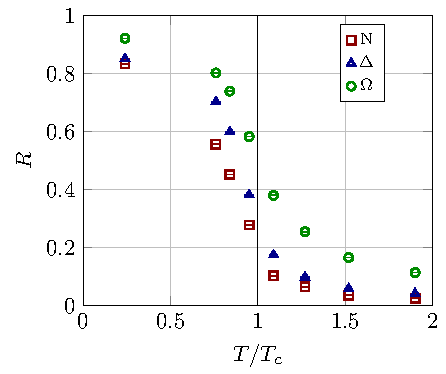
\includegraphics[width=0.8\textwidth]{figures/baryon_plot.pdf}
  \end{center}

\end{frame}

\section{Conclusion}
\frame{\sectionpage}

\section{Questions?}
\frame{\sectionpage}

\end{document}
